\usetikzlibrary{arrows,automata}

\subsection{Graph Coverage}

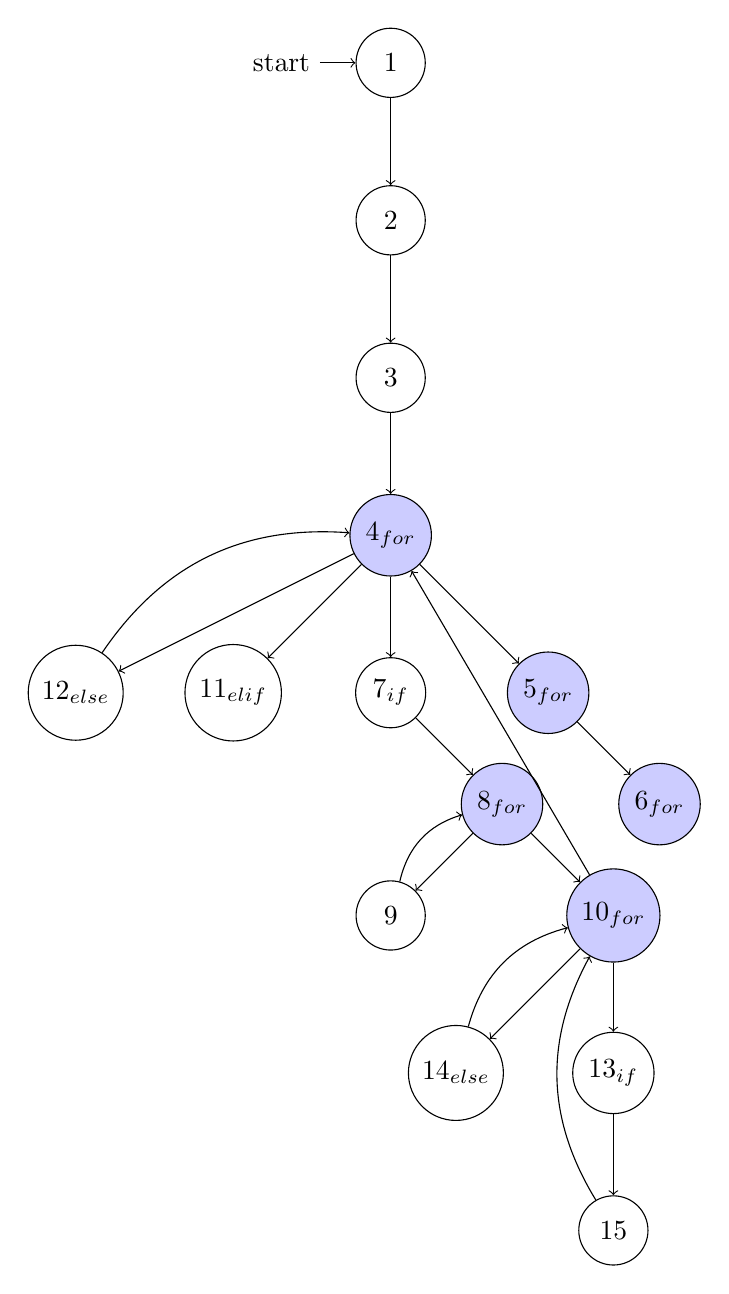
\begin{tikzpicture}[node distance=2cm, dummy/.style={circle,fill=blue!20,draw}]

% grade_document_courses = grade_document_courses or []
\node[initial,state] (1) {1};
% evaluation_results_courses = evaluation_results_courses or []
\node[state] (2) [below of=1] {2};
% publish_notifications = defaultdict(lambda: CourseLists(set(), set()))
\node[state] (3) [below of=2] {3};
% dummy for 1
\node[state, dummy] (4) [below of=3] {$4_\text{for}$};
% if course.can_publish_grades:
\node[state] (7) [below of=4] {$7_\text{if}$};
% elif len(course.textanswer_set) > 0:
\node[state] (11) [left of=7] {$11_\text{elif}$};
%TODO
% else empty
\node[state] (12) [left of=11] {$12_\text{else}$};
% dummy for 
\node[state, dummy] (8) [below right of=7] {$8_\text{for}$};
% publish_notifications[participant].evaluation_results_courses.add(course)
\node[state] (9) [below left of=8] {9};
% dummy for 
\node[state, dummy] (10) [below right of=8] {$10_\text{for}$};
% if contribution.contributor:
\node[state] (13) [below of=10] {$13_\text{if}$};
% publish_notifications[contribution.contributor].evaluation_results_courses.add(course)
\node[state] (15) [below of=13] {15};
% else empty
\node[state] (14) [left of=13] {$14_\text{else}$};
% dummy for 2
\node[state, dummy] (5) [right of=7] {$5_\text{for}$};
%TODO
% dummy for 3
\node[state, dummy] (6) [below right of=5] {$6_\text{for}$};
%TODO

\path[]
(1) edge [->] node {} (2)
(2) edge [->] node {} (3)
(3) edge [->] node {} (4)
(4) edge [->] node {} (5)
(4) edge [->] node {} (7)
(4) edge [->] node {} (11)
(4) edge [->] node {} (12)
(5) edge [->] node {} (6)
(7) edge [->] node {} (8)
(8) edge [->] node {} (9)
(8) edge [->] node {} (10)
(9) edge [->, bend left] node {} (8)
(10) edge [->] node {} (4)
(10) edge [->] node {} (13)
(10) edge [->] node {} (14)
(12) edge [->, bend left] node {} (4)
(13) edge [->] node {} (15)
(14) edge [->, bend left] node {} (10)
(15) edge [->, bend left] node {} (10);
\end{tikzpicture}
